% Figure snippets for main.tex

\begin{figure}[htbp]
\centering
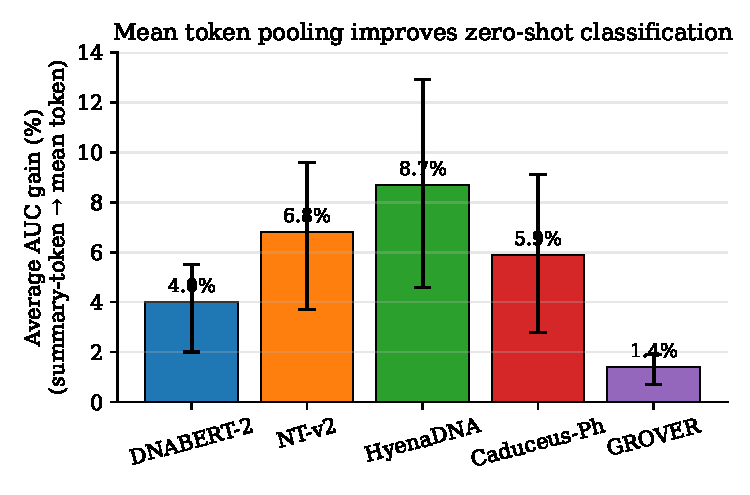
\includegraphics[width=0.75\textwidth]{figures/fig1_pooling_gain.pdf}
\caption{Average AUC gain from sentence-level summary-token pooling to mean
token pooling across 52 binary classification datasets, per model. Error bars
show the interquartile range. Mean token pooling yields consistent
improvements for every model, with the largest average gain for HyenaDNA
(8.7\%; IQR 4.6\%--12.9\%) and the smallest for GROVER (1.4\%; IQR
0.7\%--1.9\%).}
\label{fig:pooling_gain}
\end{figure}

\begin{figure}[htbp]
\centering
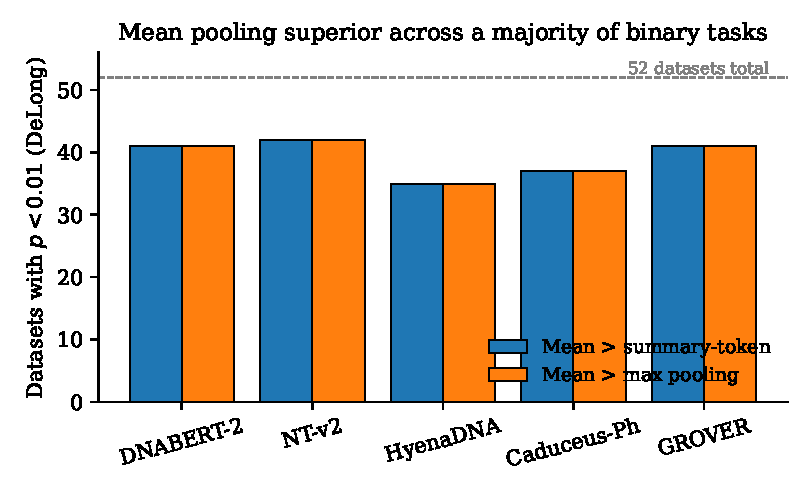
\includegraphics[width=0.75\textwidth]{figures/fig2_pooling_counts.pdf}
\caption{Number of binary classification datasets (out of 52) on which mean
token pooling was statistically superior to sentence-level summary-token
pooling (blue) or maximum pooling (orange) by a one-sided DeLong's test at
$p < 0.01$. Dashed line marks the 52-dataset ceiling.}
\label{fig:pooling_counts}
\end{figure}

\begin{figure}[htbp]
\centering
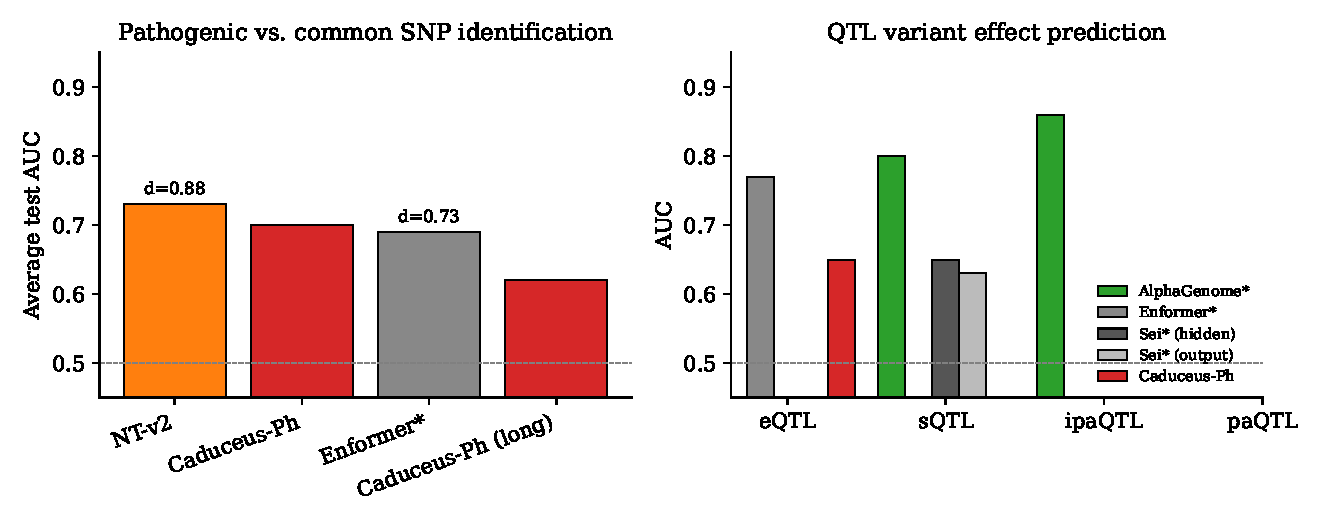
\includegraphics[width=0.95\textwidth]{figures/fig3_variants.pdf}
\caption{Variant effect quantification. Left: pathogenic vs.\ common SNP
identification (22{,}222 pathogenic, 17{,}374 common for long sequences);
Cohen's $d$ annotated where reported. NT-v2 (AUC 0.73, $d = 0.88$) surpasses
Enformer* (0.69, $d = 0.73$) and short-sequence Caduceus-Ph (0.70), while the
long-sequence Caduceus-Ph variant drops to 0.62. Right: AUC on four QTL
classes from GTEx v8 fine-mapped data (1{,}896 eQTLs, 540 sQTLs, 116 ipaQTLs,
142 paQTLs). AlphaGenome* dominates sQTL (0.80) and ipaQTL (0.86); Enformer*
reaches 0.77 on eQTL; Caduceus-Ph reaches 0.65 on eQTL; Sei* hidden states
(0.65) are nearly matched by its output tracks (0.63). Asterisks mark
non-DNA-foundation specialised models.}
\label{fig:variants}
\end{figure}

\begin{figure}[htbp]
\centering
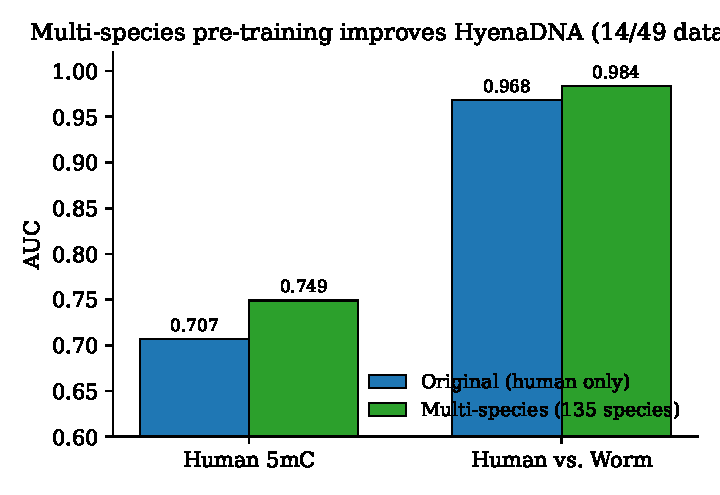
\includegraphics[width=0.7\textwidth]{figures/fig4_pretraining.pdf}
\caption{Controlled pre-training experiment. HyenaDNA re-pretrained on
DNABERT-2's multi-species corpus (135 species, 6 taxonomic categories)
improves significantly on 14 of 49 evaluated datasets. Shown are two
representative tasks with statistically significant gains: human 5mC
detection (0.707 $\to$ 0.749) and human vs.\ worm classification (0.968 $\to$
0.984). The original human-only HyenaDNA retained an advantage on 3 of 49
datasets.}
\label{fig:pretraining}
\end{figure}

\begin{figure}[htbp]
\centering
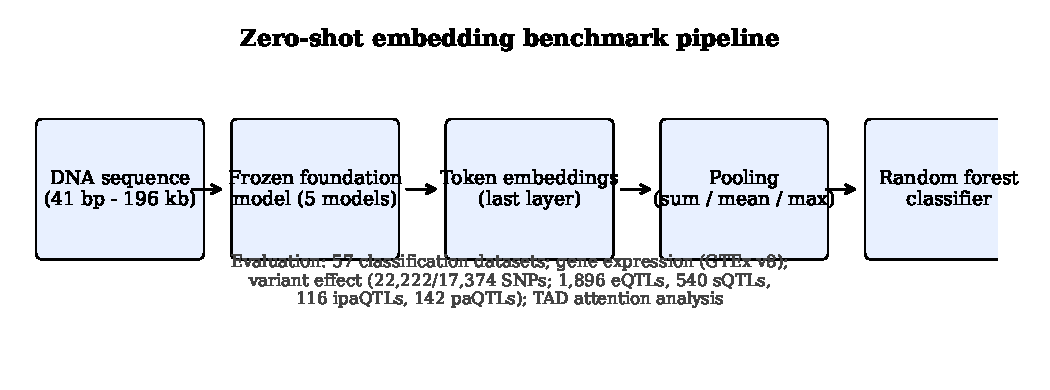
\includegraphics[width=0.95\textwidth]{figures/fig5_pipeline.pdf}
\caption{Zero-shot evaluation pipeline. DNA sequences (41 bp -- 196 kb,
task-dependent) are passed through a frozen foundation model to produce
final-layer token embeddings. One of three pooling strategies
(summary-token, mean, maximum) produces a fixed-dimensional representation
fed to a random forest classifier or regressor. The same pipeline underlies
the 57 classification datasets, GTEx v8 gene expression prediction
(610 subjects, 21{,}004 short-sequence and 768 long-sequence genes),
pathogenic SNP and QTL variant effect quantification, and attention-based
TAD analysis.}
\label{fig:pipeline}
\end{figure}
